\subsection{Experiments on Inference Latency Scaling}
\label{subsec:experiments}
In order to test the latency scaling of YANA's fully event-driven \acp{SNN} acceleration, by using our software framework, we prepare networks and data samples of different spatial and temporal sparsity levels and measure their inference time after deployment on the FPGA. 
For this, we train networks with one hidden layer of 100 \ac{LIF} units on the Spiking Heidelberg Digits (SHD) dataset.
Subsequently, we gradually increase temporal sparsity levels of the input data by uniformly dropping events. Likewise, we increase the spatial sparsity of the feed-forward layers by pruning certain percentages of weights ranking lowest in magnitude.
Note that, while we initially trained the networks until convergence to obtain realistic activity patterns, we do not take the accuracy of the networks into account. YANA's fixed-point \ac{LIF} implementation is numerically stable. Any task accuracy achieved during training in simulation is therefore preserved during inference on YANA.
In fact, the networks are meant to show the ability of YANA's architecture to leverage spatial and temporal sparsity for efficiency gains in network execution, rather than serve as a benchmark for optimally solving the SHD task.
\subsection{Results}
\begin{figure*}[t]
    \centering
    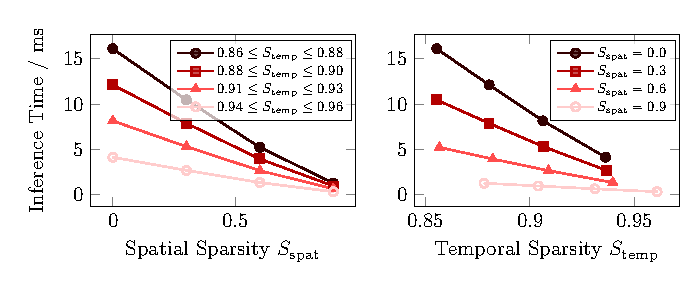
\includegraphics[width=\linewidth]{media/results.pdf}
    \caption{
    Scaling of inference time of \acp{SNN} with different spatial and temporal sparsity levels after deployment on YANA. 
    In the case of sweeping $S_\text{spat}$, $S_\text{temp}$ cannot be fixed and has to be given in a small range, since the pruning level influences hidden layer sparsity, ultimately changing the total $S_\text{temp}$.
    }
    \label{fig:exp_results}
\end{figure*}
Figure \ref{fig:exp_results} displays the results of the experiments described above. The inference time of the deployed \acp{SNN} is computed as the average of 20 samples executed on the accelerator hardware clocked at 100 MHz.
It decreases almost linearly with both increasing spatial and temporal sparsity levels of weights and data.
Since all incoming events are multicast to all connected weights, the total number of events to be processed is given by the sum of non-zero weight counts downstream of each event.
Therefore, reducing either the number of weights or the number of input events directly impacts the total number of events to be processed, effectively reducing the latency caused by the synapse and axon subcores.
Additionally, for smaller network sizes and large levels of sparsity, we observe that the inference time plateaus.
We explain this through ever fewer computation being performed in the synapse and axon cores, emphasizing the static latency ceiling of the neuron sub module and of the core control logic.
Notably, while recordings in the SHD dataset are predominantly 500ms to 1000ms long, inference times in our experiments range from 16ms to 1ms, demonstrating the speed of YANA's event-driven processing pipeline. The results showcase the considerable impact of sparsity on inference time, underpinning the importance of spike regularization and pruning techniques in \ac{SNN} application development.